\documentclass[12pt]{article}

\usepackage[portuguese,linesnumbered,ruled,vlined]{algorithm2e}
\usepackage{sbc-template}
\usepackage{graphicx,url,amsfonts}

\usepackage[brazil]{babel}
\usepackage[utf8]{inputenc}
\usepackage{hyperref}

\pagenumbering{arabic}

\sloppy

\title{Trabalho Prático de Programação Natural\\Cubo Mágico}

\author{Gabriel de Biasi\inst{1}}

\address{
Departamento de Ciência da Computação\\
Universidade Federal de Minas Gerais\\
Av. Antônio Carlos, 6627 -- Pampulha -- Belo Horizonte -- MG
\email{biasi@dcc.ufmg.br}
}

\begin{document}

\maketitle

\section{Descrição do Problema}
  O brinquedo ``Cubo Mágico'' ou \textit{Rubik's Cube} foi criado por Rubik em 1974 e distribuído comercialmente em 1980. Possui um conjunto de 26 cubos menores, 6 faces com três tipos de cubos distintos: São 4 centros, 12 meios e 8 quinas. Cada tipo cubo possui um número específico de cores, onde os centros possui uma cor, meios possuem duas cores e as quinas possuem três cores.

  É possível realizar movimentos em faces do cubo mágico sendo possível rotacionar os cubos desta face. Há 3 movimentos distintos que podem ser feitos em cada face, sendo eles: rotação horária, rotação anti-horária e dupla rotação. Logo, o cubo mágico tem um total de 18 movimentos possíveis. O objetivo do jogo é fazer com que todas as faces tenham a mesma cor. Na \autoref{fig:cube} temos na esquerda um cubo em um estado ``bagunçado'' e outro no estado concluído.


  \begin{figure}[!ht]
    \centering
    \caption{Cubo mágico bagunçado e um cubo mágico resolvido}
    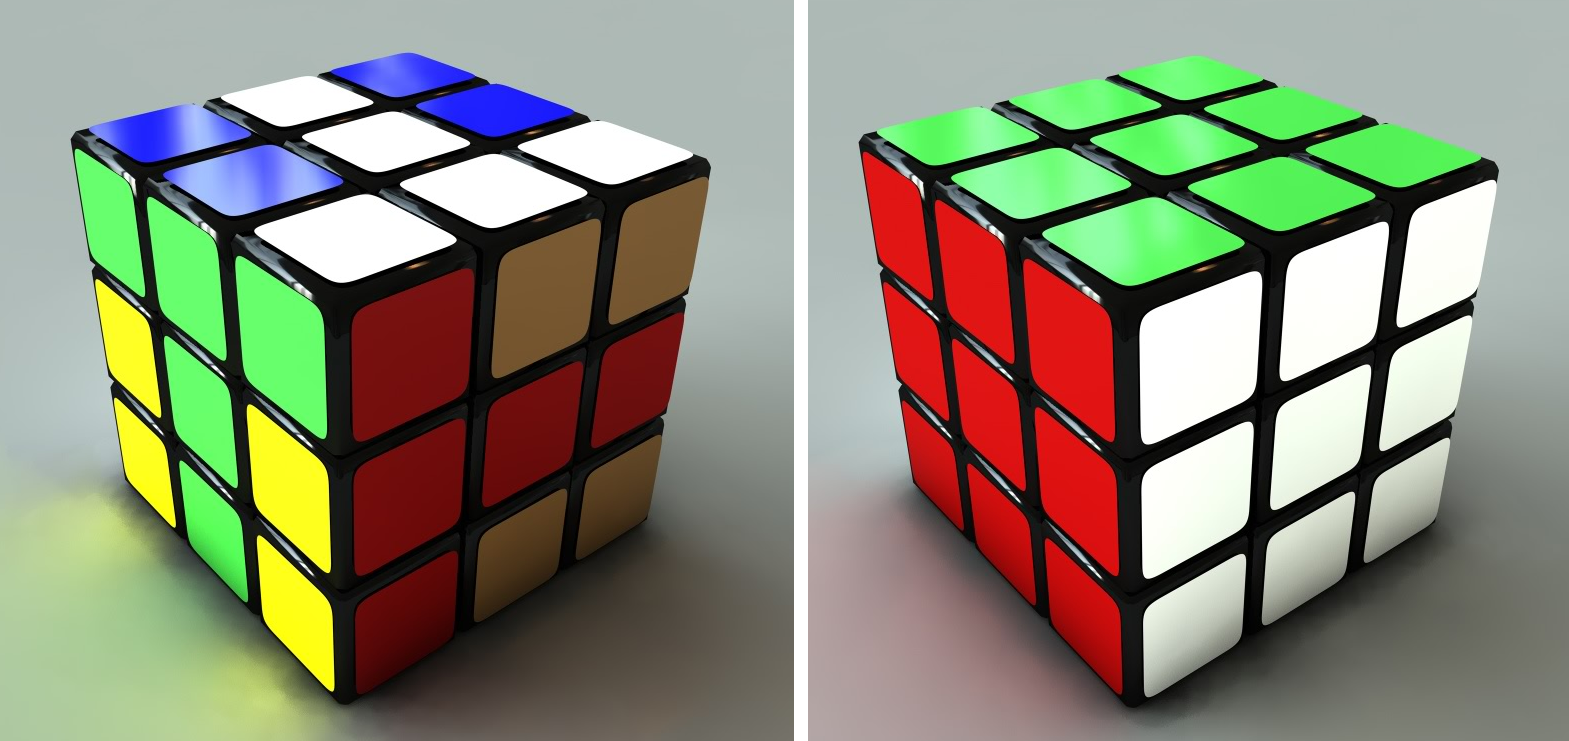
\includegraphics[scale=0.3]{images/cube.png}
    \label{fig:cube}
  \end{figure}

  Neste trabalho, é proposto um algoritmo evolutivo que tenha capacidade de resolver uma dada instância de cubo mágico colocando-o no estado resolvido e ao mesmo tempo buscando minimizar a quantidade de movimentos necessários.

\section{Metodologia}
  Para alcançar o objetivo do jogo, foi utilizado como base um método de resolução criado pelo professor \textit{Morwen Thistlethwaite}, onde o espaço de buscas de soluções é categorizado e então o cubo precisa ser levado de uma categoria para a próxima utilizando apenas os movimentos permitidos da categoria atual.

  \subsection{Categorias do Cubo}
  Thistlethwaite criou 5 categorias, que descreve o tão próximo um cubo mágico está da solução. Os movimentos que são permitidos em cada categoria que permitem levar para a próxima são as seguintes:

  \begin{table}[ht]
      \centering
      \caption{Movimentos permitidos em cada categoria}
      \begin{tabular}{|c|c|}
        \hline
        \textbf{Categoria} & \textbf{Conjunto de Movimentos Permitidos}  \\ \hline
            G0             &  $(F, R, U, B, L, D)$           \\ \hline
            G1             &  $(F, R, U, B, L2, D2)$         \\ \hline
            G2             &  $(F, R, U2, B2, L2, D2)$       \\ \hline
            G3             &  $(F2, R2, U2, B2, L2, D2)$     \\ \hline
            G4             &  $\emptyset$                    \\ \hline
      \end{tabular}
  \end{table}

  \cite{thistlethwaite}.

\section{Descrição Geral da Implementação}
  lala

\section{Execução dos Experimentos}
  lala

\section{Conclusão}
  Neste trabalho.

\bibliographystyle{sbc}
\bibliography{ref}

\end{document}
